	\documentclass[12pt]{report}

	\usepackage[utf8]{inputenc}
	\usepackage[T1]{fontenc}
	\usepackage[french]{babel}
	\usepackage[french]{datetime}
	\usepackage[top=2cm, bottom=2cm, left=2cm, right=2cm]{geometry}
	\usepackage{makecell, hyperref, listings, amsmath, amssymb, color, titlesec, graphicx, titling, xcolor, tikz, wrapfig}
	\titleformat{\chapter}
	  {\normalfont\LARGE\bfseries}{\thechapter}{1em}{}
	\titlespacing*{\chapter}{0pt}{3.5ex plus 1ex minus .2ex}{2.3ex plus .2ex}
	\makeatletter
	\@addtoreset{chapter}{part}
	\makeatother 

	\newcommand{\tb}[2]{\textbf{\color{#1}{#2}}}

	\hypersetup{
		colorlinks=true,        % false: boxed links; true: colored links
		linkcolor=blue,        % color of internal links (change box color with linkbordercolor)
		citecolor=black,        % color of links to bibliography
		filecolor=black,        % color of file links
		urlcolor=cyan           % color of external links
	}
	
    \begin{document}
    \begin{figure}
		\centering
			
\includegraphics[height=3cm]{figures/LogoFDS.png}
		    
\includegraphics[height=3cm]{figures/LogoUM.png}
	\end{figure}
	\bigskip
	\begin{figure}
		\centering
    
\includegraphics[height=6cm]{figures/qr.png}
	\end{figure}
	\bigskip			
	
	
	\title{HLIN405 - Projet de Programmation \\
	L2 - Licence Informatique \\
	Faculté des Sciences de Montpellier \\}
	\author{Cédric Cahuzac,\\ Charlotte Fabre,\\ Robin L'Huillier,\\ Lorenzo Puccio,\\ Nicolas Ruiz,\\ \bigskip Référent: Vincent Boudet}
	\date{\today}

		\begin{titlingpage}
			\begin{center}
				\vspace{5cm}
				\begin{LARGE}\thetitle\end{LARGE}
			    \vspace{2cm}
				\begin{large}\theauthor\end{large} \\
				\vspace{2cm} 
				\thedate
			\end{center}
		\end{titlingpage}
		\tableofcontents
		\listoffigures

		\chapter{Introduction}
		\par
        Ce rapport décrit le déroulement de notre projet de programmation web, ainsi que son fonctionnement et ses spécificités. Ce projet avait pour objectif de nous permettre d’utiliser les connaissances et aptitudes que nous avons acquises depuis le début de nos études d’informatique et plus particulièrement dans le cadre des cours d’HLIN304, HLIN405 et HLIN408.
		    
	    \bigskip
		\par
        Pour rappeler brièvement le sujet, il s’agissait de développer un site de gestion de tournoi et sa base de données associée. Nous avons donc dû, dans un premier temps, choisir sur quoi porteraient les tournois gérés par notre site. Nous nous sommes mis d’accord sur le basketball pour plusieurs raisons. D’abord, un tournoi sportif (plutôt que festif) semblait plus approprié au travail que nous voulions produire : des règles plus strictes nous permettaient de commencer avec un cadre clair. Parmi les nombreuses activités, nous avons choisi le basketball car c’est un sport d’une part assez populaire pour donner un intérêt à notre site, d’autre part assez intéressant pour nous permettre de laisser libre cours à notre volonté de rajouter des fonctionnalités. Ainsi, le basketball peut être joué dans plusieurs types de tournois, et a un nombre de joueurs par équipe assez limité pour ne pas nous freiner dans notre programmation. Un autre choix important que nous avons fait est celui de proposer un site accessible et simple d’utilisation pour permettre aux supporters de conserver le contact avec les tournois, particulièrement au cours d’une crise sanitaire où il est difficile d’accéder aux rencontres en personne.
		    
	    \bigskip
	    \par
	    À partir de ces choix déterminants et de notre nom d’équipe, les Suricates (Meerkat en anglais), nous avons pu donner naissance à Meerketball, un site web pratique qui permet de gérer les tournois de basketball, leurs équipes et leurs rencontres. Pour en savoir plus sur la création et la programmation de ce projet, ce rapport regroupe cinq parties.
		    
	    \bigskip
	    \par
	    La première partie décrit la \textbf{gestion de notre groupe}. Nous y décrivons la façon dont nous nous sommes organisés à cinq pour fournir un travail le plus complet possible. Nous y parlons aussi des outils dont nous nous sommes servis pour rendre notre collaboration efficace au sein des différentes parties du projet.
		    
	    \bigskip
	    \par
	    La seconde partie est celle de la description de notre \textbf{base de données} (ou BDD). En tant que base fondatrice du site, la BDD a été la première étape de notre travail de groupe. Elle est aussi la phase sur laquelle nous avons passé le plus de temps en groupe, car il était essentiel que nous l’ayons tous bien en tête.
		    
	    \bigskip
	    \par
        La troisième partie concerne l’\textbf{architecture} de Meerketball, c’est-à-dire la façon dont les différentes parties isolées ont été agencées et regroupées afin de fournir un site final utilisable, centré autour d’une page d’accueil simple.
		    
        \bigskip
        \par
        La quatrième et dernière partie porte sur les \textbf{particularités techniques} que nous avons ajoutées à notre projet. Ce sont ces fonctionnalités qui en font un site unique et un produit fini.

        \chapter{Gestion de Groupe}
        \par
        Le début du projet pour notre groupe était en décembre 2020, au moment du choix des différents membres. L’important était surtout de savoir identifier les forces et les faiblesses de chacun, afin de pouvoir facilement se compléter et s’aider sur les différentes tâches à venir. C’est notamment ce diagnostic qui a permis de diriger chacun des membres du groupe vers une position définie dans le projet. Par exemple, Robin L’Huillier a été à l’origine de beaucoup d’initiatives de communication vers notre tuteur et de prise de décisions internes à notre groupe, prenant facilement la place de chef de projet. Mais bien qu’il soit chef de projet, chacune de ses propositions devait être approuvée par la grande majorité avant d’être conduite, permettant ainsi de faire valoir nos forces et nos faiblesses et planifier nos objectifs sur le court et long terme.
        
        \bigskip
        \par
        Pour communiquer facilement, nous avons utilisé la plateforme de discussion Discord : en plus de sa facilité d’utilisation et son système de serveurs séparés permettant une discussion totalement privée, elle permet aussi d’inclure du code d’un langage à spécifier dans un message. Cela s’est avéré très pratique lors de nos premiers essais en PHP et SQL car les différents termes dans le code étaient colorés comme dans la plupart des éditeurs de texte inclus dans une API, rendant la compréhension du travail de chacun plus simple.
        
        \bigskip
        \par
        Afin de pouvoir travailler efficacement, nous avons utilisé le domaine GitLab fourni par la Faculté des Sciences et nous avons créé notre répertoire de projet à partir d’ici. Nous étions peu à savoir comment utiliser GitHub Bash avant le début du projet, mais nous avons rapidement pu mettre notre savoir en commun afin de préparer l’équipe avant le début du semestre pair. De plus, l’unité d’enseignement HLIN408 – Techniques de communication et conduite de projets comprend un cours assez complet sur GitHub et son utilisation.
        
        \bigskip
        \par
        Enfin, la rédaction de ce rapport nous a permis d’utiliser la plateforme en ligne Overleaf, permettant d’éditer un fichier LaTeX en collaboration. LaTeX est un langage de programmation spécialisé dans le traitement de texte. Plusieurs logiciels peuvent prendre en charge le langage LaTeX, dont Overleaf. La complexité du langage est équilibrée par la diversité du contenu que comprend celui-ci : une grande variété d’extensions permet d’enrichir un document d’une manière plus flexible encore que ce qu’offrent les logiciels de traitement de texte classique. L'unité d'enseignement HLIN408 - Techniques de communication et conduite de projets comprend également un cours sur LaTeX.
        
        \bigskip
        \par
        On distingue plusieurs phases du projet. La phase préparatoire est une phase précédant le semestre pair afin de pouvoir s’organiser sur les toutes premières tâches du projet et notamment leur répartition. La vraie première phase du projet permet de conceptualiser et implémenter la base de données, puis l’améliorer si besoin. La deuxième phase du projet concerne la répartition de chacun des formulaires obligatoires pour chacun des membres du groupe, ainsi que la création d’une première version. La troisième phase concerne la finalisation de ces formulaires, à savoir l’ajout de contenu supplémentaire dans ces formulaires. La quatrième phase débute en même temps que la troisième phase et concerne principalement la réalisation de formulaires supplémentaires. La cinquième et dernière phase concerne le débogage de tous les formulaires et la rédaction du rapport final.
        
        \bigskip
        \par
        \hypertarget{bdd-retour-gestion}{}
        Le mode de travail dans le groupe s’est organisé ainsi : nous travaillons chacun de notre côté jusqu’à une réunion le mercredi de chaque semaine. Cette réunion est organisée sur le créneau de travail en groupe commun à tous les groupes de L2 Informatique de 15h à 18h15. Quand un membre du groupe a fini de travailler sur un ou plusieurs fichiers, nous consultons le reste du groupe afin de vérifier que l’on ne perd pas de progression sur ces fichiers. Si le fichier n’a été édité par personne d’autre dans la même période de temps, nous utilisons la fonction « push » de GitHub et envoyons les modifications sur le dossier en ligne du projet. \hyperlink{annexe-gestion}{Le nombre de commits sur la durée projet est donné en annexe}. Nous n'avions pas créé de branches pour chacun des membres, bien qu'en rétrospective nous aurions dû afin de simplifier notre mode de fonctionnement. Comme dit plus haut, nous prenons toutes les décisions ensemble et essayons toujours de trouver un compromis ou de s’aider pour faire avancer le groupe dans toutes les circonstances (difficultés techniques, membre malade, etc.). Le travail fourni a été exclusivement en distanciel depuis nos propres machines.
        
        \bigskip
        \par
        Pendant la cinquième et dernière phase du projet portant en majorité sur le débogage de nos formulaires, nous avons utilisé Google Sheets afin de rendre compte des bugs sur les formulaires des autres. Une ligne dans un tableur est séparée en deux colonnes: l'une consacrée au bug lui-même et sa nature, l'autre consacrée au contexte derrière l'apparition du bug. \hyperlink{annexe-gestion}{L'affichage d'un de ces tableurs de débogage est donné en annexe}. Quand un bug est corrigé, on coche la case à côté de la ligne, ce qui raye son contenu et signale aux autres membres que le bug est corrigé.
        
        \bigskip
        \par
        Pendant les différentes phases du projet, nous avons fixé plusieurs objectifs sur le court terme et le long terme. Parmi ces différents objectifs, beaucoup ont été fixés sur le créneau horaire de 15h à 18h15 détaillé dans le paragraphe précédent. Notamment, le premier jet des cinq formulaires principaux du site avait été fixé au mercredi 3 mars. D’autres objectifs comme la première esquisse de la base de données ont été fixés en dehors de ce créneau, même sans date de fin explicite. Enfin, une dernière catégorie d’objectifs à atteindre a été fixée selon les réunions de mise au point avec notre tuteur de projet ; pour les mois de mars et d’avril où la réalisation du projet était dans sa troisième et quatrième phases de projet, nous avons pris contact avec notre tuteur afin de montrer notre progression dans le projet. Cela a été très utile d’avoir son point de vue puisque d’habitude, chacun ne consulte personne d’autre que les membres du groupe lors d’un avis à donner sur les fonctionnalités du site. Ainsi, il fallait qu’avant chacune des trois réunions avec notre tuteur (17 mars, 7 avril et 22 avril), tous nos objectifs de court terme et de long terme soient atteints.
        
        \bigskip
        \par
	    \hyperlink{annexe-gestion}{Nous avons créé un diagramme de Gantt}
         avec le logiciel Gantter pour Google Drive, qui rend compte de l’organisation globale du projet et du temps passé sur les différentes phases du projet expliquées plus haut.

        \chapter{Base de Données}
        
        \par
        Le premier schéma de relations d'entités de notre site de tournoi ne contient pas les entités arbre et championnat, dont nous parlerons plus tard. Elles seront explicitées dans les second et  troisième schémas, et correspondent à la mise en œuvre d'un type particulier de tournoi. 
        
        \begin{figure}[!h]
			\centering
				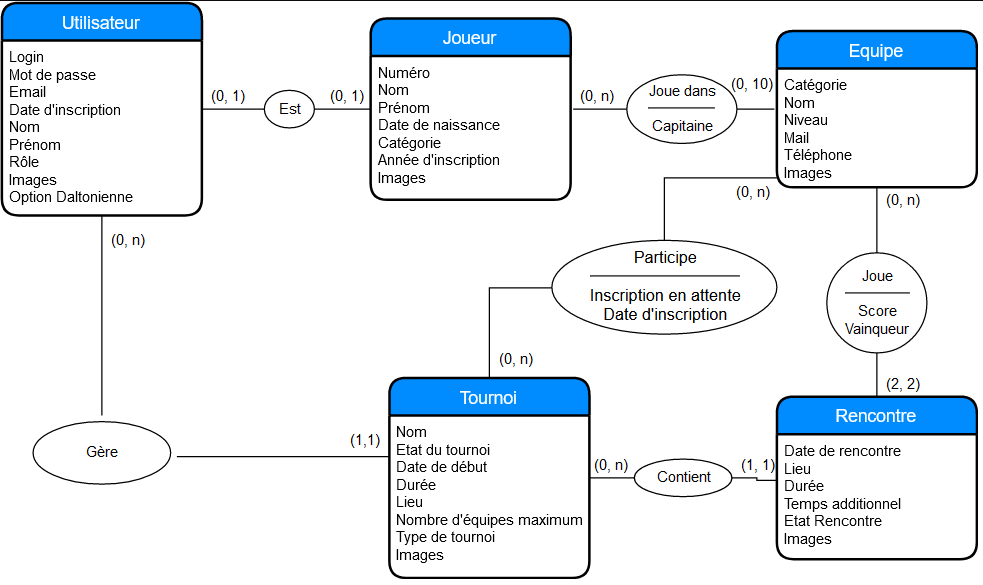
\includegraphics[height=9cm]{figures/bdd-rapport-1.png}
			\caption{Schéma de relation entité-association}
		\end{figure}
		
        \par
        La première entité est l'utilisateur, ainsi que toutes ses informations. Il peut être joueur, mais aussi avoir un rôle qui définit sa position au cœur du site: "utilisateur", "gestionnaire" ou "administrateur". L'administrateur a accès à toutes les fonctionnalités, l'utilisateur peut s'inscrire et voir le déroulement des tournois, tandis que le gestionnaire peut gérer un ou plusieurs tournois (tandis qu'un tournoi n'est géré que par un gestionnaire).
        \par
	    Le joueur peut donc être utilisateur ainsi qu'être membre d'une ou plusieurs équipes. Les équipes comprennent de 0 à 10 joueurs, dont l'un est capitaine. 
	    \par
	    L'entité tournoi contient entre 0 et n rencontres, et une liste d'équipes. La liste d'équipes contient pour chaque équipe un booléen : chaque équipe demande à s'inscrire à un tournoi, et le gestionnaire les accepte ou rejette. Le lien entre les rencontres et le tournoi sera fait ultérieurement par une entité dépendante du type de tournoi.
	    \par
	    L'entité rencontre est liée aux équipes par une cardinalité (2, 2): une rencontre est jouée par deux équipes, qui obtiennent chacune un score, et est gagnante ou perdante. Nous pouvons observer que dans la mise en œuvre de la base de données, puisque ce lien est constant, les références aux équipes, scores et vainqueur ont intégré la table rencontre. 
	    \par
	    Nous avons hésité quant au comment représenter les listes d'équipes et de joueurs dans une base de données. Initialement, nous avons tenté de créer des tables contenant autant d'attributs "équipeX" que le maximum d'équipes que nos fonctionnalités pourraient accepter, mais cela s'est avéré peu pratique à manipuler. Nous avons alors choisi de représenter les listes d'équipes et de joueurs au travers de deux tables liées par des références aux tables concernées. Pour les listes d'équipes, chaque tuple référence une équipe et un tournoi, permettant ainsi de trier dans un sens et dans l'autre aisément tous les tournois auxquels participe une équipe, ou toutes les équipes participant à un tournoi. 
	    \par
	    Dans un premier temps, nous avons choisi de nous concentrer sur le type de tournoi "Coupe", le type correspondant aux critères attendus, à savoir une représentation en arbre. Plus tardivement, nous avons ajouté un second type de tournoi, le "Championnat", dont l'information est contenue dans une seconde table construite de manière similaire à la table "Arbre" et que nous allons détailler dans ce second schéma. 
        
        \begin{wrapfigure}{L}{8cm}
			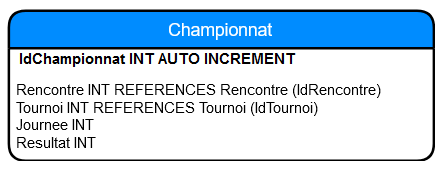
\includegraphics[width=8cm]{figures/bdd-rapport-2.png}
		\end{wrapfigure}	    
	    
	    \par
	    Dans un tournoi "Championnat", l'interface entre les entités tournoi et rencontres est représentée par la table ci-contre. Chaque entrée référence donc les deux tables, et contient deux informations supplémentaires: Journée et Résultat. Les championnats sont en effet organisés par journée, et à la différence des coupes, acceptent des matchs se soldant par une égalité entre les deux équipes. Le résultat symbolise cela, en codant l'information en fonction de l'équipe jouant à domicile (représentée par l'équipe 1 dans la table rencontre). 
	    \bigskip
	    
	    \par
	    \hypertarget{bdd-retour-annexe}{}
	    \hyperlink{annexe-bdd-tableref}{Nous pouvons voir en annexe}
	    le schéma qui nous a servi de référence durant la phase de programmation. Lors de sa conception n'y figurait alors pas encore la table "Championnat", dont nous ne savions pas encore si nous l'insérerions. Afin de manipuler la base de données, nous avons d'abord utilisé mysqli, puis sommes passés à PDO. Lors de l'implémentation de la base de données, nous avons décidé que toutes les clés primaires seraient insérées en auto-increment, c'est-à-dire que nous ne les préciserions pas lors de l'ajout de nouvelles valeurs; que les booléens seraient enregistrés sous forme de BIT(1), de valeur 0 ou 1.
	    \par
	    La modélisation des rencontres d'un tournoi "Coupe" se fait au travers de la table Arbre, qui référence le tournoi, les équipes participant à une rencontre, et une rencontre, mais aussi elle-même. Chaque nœud de l'arbre binaire correspond à une rencontre. Ses parents sont les noeuds/rencontres du tour précédent, et son fils est le noeud/rencontre du tour suivant qu'il engendre. Un attribut Hauteur permet d'enregistrer la hauteur du noeud, 0 correspondant à la finale, 1 à un noeud de demi-finale, etc. 
	    \par
	    Nous pouvons remarquer a priori que plusieurs attributs pourraient ne pas être contenus dans la table Arbre: Equipe1/Equipe2 ainsi que Hauteur.	Concernant Hauteur, elle pourrait être obtenue après plusieurs requêtes ou un calcul sur tous les tuples d'Arbre pour un Tournoi donné. Ce serait coûteux à mettre en place, plus que de retenir l'information dans la table. Quant à Equipe1/Equipe2, les deux attributs paraissent redondants vis-à-vis de la table Rencontre, qui les contient aussi. C'est une question de conception: dans un tournoi de type "Coupe", la table Arbre est construite avant que les rencontres soient créées, ce qui demande de retenir l'emplacement des équipes. Et si nous mettions en place d'autres types de tournoi, ou des rencontres amicales, la table Rencontre devrait contenir l'information. Nous avons donc fait sciemment le choix d'une apparente redondance sur ces deux attributs. 
        
        \chapter{Architecture}
        \par             
	    Un squelette commun est intégré dans toutes les pages par le truchement de la fonction PHP include. Il  est constitué de:
	    \begin{itemize}
        \item{un bandeau coulissant (via un bouton amovible),}
        \item{un bandeau haut contenant les boutons permettant de se déplacer sur le site,}
        \item{ un bandeau bas contenant l’assistance, un bouton retour vers le bandeau haut,}
        \item{une page «connexion.php» permettant la connexion vers la base de données.}
        \end{itemize}
       L’interface utilisée entre les pages et la base de données est PDO car elle est indépendante du système de gestion de base de données.   
        \bigskip
       
       \par
	   La page d’accueil du site «index1.php» affiche, grâce à la fonction include, les pages «carousel2.php»,«carousel2Resp.php» et «ListeDesTournois.php».
       Le carrousel situé sous le bandeau haut dans la page d’accueil est construit à partir des pages «carousel2.php» et «carousel2Resp.php», le fichier style.css se charge d’en afficher un des deux selon la taille de l’écran.
       La page «listeDesTournois.php» visible depuis l’accueil conduit vers les pages «AffichageTournoiChoisit.php» et «Championnat.php» qui offrent l’accès aux arbres des tournois ainsi qu’aux classements des championnats.
       \bigskip
       \par       
       La page de création des tournois «CreationTournoi.php» communique avec la base de données en utilisant les fonctions php prepare, query, execute qui prennent pour paramètres  les requêtes SQL Update, Select et Insert Into pour y insérer des valeurs nécessaires au bon fonctionnement du site (changement éventuel du statut d’un utilisateur, nom du tournoi, type du tournoi, durée du tournoi, etc.) . Cette page est donc accessible uniquement aux administrateurs. La vérification est faite grâce à la variable super globale \$\_SESSION, utilisée comme matrice et initialisée lors de la connexion sur la page «LoginUtilisateur.php».
       \bigskip
       \par
 	   La page «LoginUtilisateur.php» récupère les informations de la base de 
 	   données par les fonctions prepare, execute prenant en paramètre des 
 	   requêtes SQL Select afin de vérifier l’adéquation entre l’identifiant 
 	   fourni et le mot de passe saisi. Ces informations inscrites dans la base 
 	   de données  y ont été insérées lors de l’inscription du compte issue de 
 	   la page «Inscription.php». Une ancre HTML dans le bandeau haut lui 
 	   permet d’afficher les hyperliens vers les pages «Inscription.php» et 
 	   «LoginUtilisateur.php».
       Un utilisateur connecté voit affiché l’hyperlien menant à la page utilisateur  «CompteUtilisateur.php» contenant toutes ses informations personnelles. Ces informations viennent de la base de données ; elles sont obtenues par l’intermédiaire d’une requête SQL Select dans une fonction php prepare et peuvent être modifiées par la transmission des informations de changement assurée par la variable super globale \$\_POST et le formulaire HTML action qui mène vers la page «ModifInfosPerso.php». Les modifications fonctionnent de manière analogue. Les informations de \$\_POST sont vérifiées par des requêtes SQL Select dans la fonction php query, puis modifiées par des requêtes SQL Update dans la fonction php exec.
       La page utilisateur permet aussi de se désinscrire du site en supprimant la ligne de la base de données contenant les informations propres à l’utilisateur via la fonction php exec et la requête SQL Delete. Cette requête utilise le login de l’utilisateur qui est un attribut unique récupéré grâce à la variable super globale citée supra.  \bigskip
       \par
	   La page «Equipe.php» est disponible pour l’ensemble des utilisateurs connectés. Cette information est donnée par \$\_SESSION. Elle inscrit dans la base de données, par la fonction php exec dont le paramètre est une requête SQL Update, l’ensemble des joueurs d’une équipe, ainsi que son capitaine. Son affichage dépend des informations qu’elle récupère via \$\_POST.
	   \bigskip
       \par
	   La page «Preinscription.php», accessible elle aussi à l’ensemble des utilisateurs connectés, vérifie par le même mécanisme pré-inscrit les équipes dans un tournoi grâce aux informations stockées dans \$\_SESSION et \$\_POST.
       \bigskip
       \par
   	   La page «GestionTournoi.php» affiche par la fonction include la page 
   	   «GestionTournoiSynthese.php», laquelle par un formulaire HTML lui 
   	   répond en l’appelant.
       L’affichage de l’onglet synthèse se fait par la récupération des informations la concernant dans \$\_SESSION. Une fois affichées, les informations que la synthèse procure dépendent de celles qui sont récupérées par une requête SQL Select dans une fonction php query. La synthèse permet entre autres de modifier des données de la base de données par une requête SQL Update, paramètre de la fonction php exec. Elle permet aussi de faire par les mêmes mécanismes les actions décrites ci-dessous. Ces mécanismes concernent les tournois à élimination directe.
       La validation des équipes possède son propre onglet. Si une équipe est validée, les informations de la base de données sont modifiées au moyen d’une requête SQL Update; à l’inverse, si l’équipe est rejetée, la demande d’inscription est supprimée de la base de données au moyen d’une requête SQL Delete. Ces 2 requêtes sont dans une fonction php exec.
       Les scores sont gérés par une requête SQL Update, paramètre de la fonction php exec, ainsi que des variables \$\_POST.
       Enfin, le passage au tour suivant modifie les informations de la base de données via une requête SQL Update elle aussi dans la fonction exec, et insère les nouveaux nœuds d’un tournoi avec une requête SQL Insert Into dans la fonction php query.
       L’insertion des rencontres est exécutée par une fonction php query qui prend une requête SQL Insert Into. Les informations insérées proviennent de \$\_POST. 
       Le fonctionnement de la page «GestionTournoi.php» dépend de \$\_SESSION qui renseigne le type de tournois. En effet, un championnat n’est pas géré de la même manière qu’un tournoi à élimination directe. L’ensemble des nœuds d’un championnat sont déjà générés automatiquement par une requête SQL Insert Into à l’intérieur de la fonction php exec qui, elle-même, se situe dans la page «CreationTournoi.php»; les championnats n’ont donc pas besoin de passer au tour suivant. L’ensemble des rencontres est fixé par le truchement d’une requête SQL Update d’une fonction php exec qui se déclenche dès que le nombre d’équipes requis du championnat est atteint via la même requête Update que celle des tournois à élimination directe citée plus haut.   
       La gestion d’un tournoi n’est disponible que pour un administrateur qui a accès à l’ensemble des tournois ou un gestionnaire qui ne verra que ses tournois grâce à la requête SQL Select de la fonction php query, qui utilise \$\_SESSION fournissant le login.
       \bigskip
       \par
	   La déconnexion d’un utilisateur détruit la session en cours grâce à l’appel à la fonction php session\_destroy. La page «Deconnexion.php» communique donc indirectement avec l’ensemble des autres pages en effaçant les informations contenues dans \\ \$\_SESSION.
       \bigskip
       \par
	   Enfin, le bandeau coulissant latéral appelle par la fonction php include les 5 carrousels disponibles sur les pages «carousel3.php», «carousel4.php», «carousel5.php», «carousel6.php»,\\ «carousel7.php».
       Les images de ces carrousels proviennent de la base de données par l’intermédiaire de requêtes SQL Select effectuées par la fonction php query. Elles ont pour finalité de servir de lien vers la page qui affichera l’avancée du tournoi correspondant à l’image.
       
       
        \chapter{Particularités Techniques}
        
        \section{Cadre général}
        \subsection{Navigation}
\par
Le menu hamburger (trois traits horizontaux parallèles), permet de regrouper les différentes pages, les accès aux formulaires, la FAQ, la page d’assistance et la page d’administration pour avoir accès aux fonctionnalités de développement telles la réinitialisation automatique de la BDD via notre fichier de démonstration, ou bien le formulaire pour hacher les mots de passe.
        \subsection{Redirections}
\par            
Pour accéder au site côté client, il faut ouvrir le fichier index.html à la racine du projet. Ce fichier ne contient qu’une redirection vers un fichier index1.php dans le dossier nommé CadreStatique, structurant l’ensemble de l’application web. Il a été fait ainsi en raison de WAMP et autres outils qui sont configurés pour ouvrir par défaut tout fichier intitulé index et ne donnant de ce fait plus accès au reste des fichiers. Par la suite, des redirections internes aux formulaires, et autres liens vers l’accueil ont été créés, et il est devenu risqué de changer le nom et le chemin de index1.php, donc cette astuce de redirection garantit l’absence d’un oubli d’édition des liens/redirections.
\bigskip
\par    
Le logo et le nom du domaine (Meerketball) redirigent vers l’accueil, et le bouton Top du footer est une ancre vers le haut comme son nom l’indique. Le titre principal de la page est quant à lui un lien vers lui-même pour actualiser la page.
\bigskip
\par    
L’affichage des éléments des liens et menus varie selon l’état de connexion et le rôle de la personne inscrite. Une fois l’inscription ou la connexion et leur redirection automatique effectuées, prennent place les liens de déconnexion et le login de l’utilisateur, qui est en fait un lien vers les options du compte où ce dernier peut modifier les informations saisies lors de l’inscription ; comme l’aspect visuel du site, ou supprimer son compte. Cette dernière action supprime de la BDD l’utilisateur, le redirige vers déconnexion, détruit la session PHP et redirige à son tour vers l’accueil.
        \subsection{Accessibilité et autorisations}
\par
\hyperlink{annexe-access-et-auto}{Voir annexe.} 
\hypertarget{retour-access-auto}{}
        \subsection{Unifier l'application Web}
\par
\hypertarget{retour-unifier}{}
\hyperlink{annexe-unifier-web}{Voir annexe.} 
\newpage
        \section{Langage et syntaxes}
        \subsection{CSS : Cascading Style Sheets}
        \subsubsection{Rendu visuel (+ responsive)}
\par
\hypertarget{retour-rendu-visuel}{}
\hyperlink{annexe-rendu-visuel}{Voir annexe.}
        \subsection{PHP : PHP Hypertext Preprocessor}
         \subsubsection{Affichage des tournois}
\par
La génération d’arbres est entièrement gérée en PHP et HTML et non pas à l’aide d’une librairie JS prête à l’emploi. Les cases sont des div dont le contour est affiché, de même que les traits de jonctions, dont seul le contour haut ou bas ou latéral est affiché (\hyperlink{fig-arbre1}{Arbre 1}).
 \begin{figure}[h]
 \hypertarget{fig-arbre1}{}
			\centering
				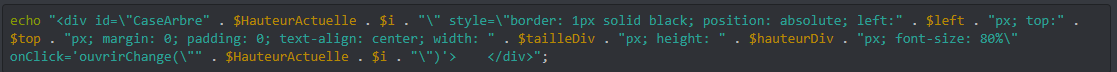
\includegraphics[width=17cm]{figures/pt-arbre1.png}
			\caption{Arbre 1}
\end{figure}
\bigskip
\par
Le calcul du placement des div est fait par rapport à la hauteur en cours (selon l’avancement du tournoi) et du nombre de cases par hauteur correspondante. Et grâce à un certain nombre d’autres variables, l’arbre est relativement responsive, conservant ainsi ses proportions si la longueur ou la largeur donnée venait à être modifiée. Sur chaque case est appliqué un tooltip (infobulle) et le CSS adéquat, couleur pour les gagnants, réaction au passage de la souris (hover), etc (\hyperlink{fig-arbre2}{Arbre 2}).
\begin{figure}[h]
\hypertarget{fig-arbre2}{}
			\centering
				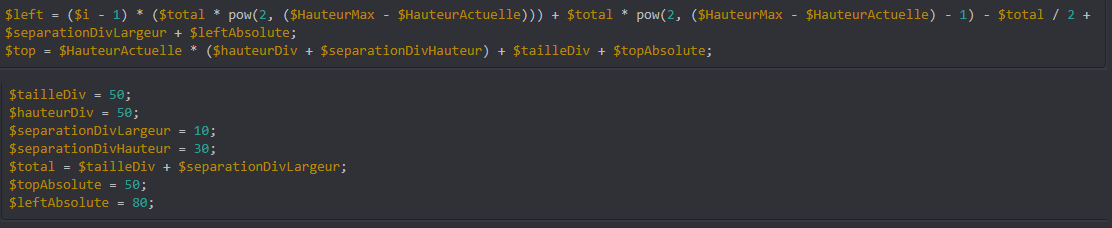
\includegraphics[width=17cm]{figures/pt-arbre2.png}
			\caption{Arbre 2}
\end{figure}
        \subsubsection{Formulaires}
\par
\hypertarget{retour-formulaires}{}
\hyperlink{annexe-formulaires}{Voir annexe.} 
        \subsubsection{Upload}
\par                
La possibilité de téléverser (upload) des images a été mise en place lors de la création des tournois/équipes. Une variable gérant les exceptions est initialisée avant le processus d’envoi. Si aucune image n’est chargée, la variable image sera celle par défaut. Si une image est chargée et le tournoi créé, le chemin est généré, sauf si l’image est vide ce qui déclenche une exception de format (getimagesize). Si l’image est déjà présente (filename et filesize : nom et tailles différentes), seul le champ correspondant dans la BDD sera initialisé/modifié, sans avoir à faire d’upload surnuméraire. Enfin, si aucune exception n’est déclenchée, en plus de l’action sur la BDD, l’image est chargée dans le dossier correspondant (ImagesUtilisateur/Tournois).
\subsubsection{Carrousels}
\begin{wrapfigure}{l}{0.5\textwidth}
\hypertarget{fig-carrousel7}{}
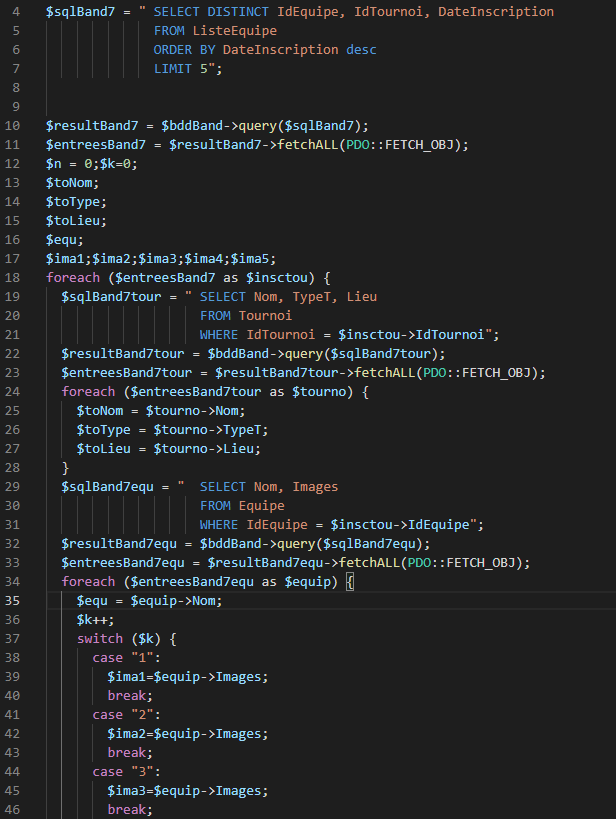
\includegraphics[width=0.95\linewidth]{figures/pt-carrousel7.png} 
\caption{Carousel 7}
\end{wrapfigure}
\par
À la différence des carrousels centraux (carousel2) de l’accueil, les carrousels (carrousels 3 à 7) du bandeau latéral sont dotés d’un appel à la base de données pour afficher les images correspondantes aux informations présentes. L’implémentation est plus élégante et ne demande pas aux développeurs de modifier le code pour changer les images. Cependant la conception n’est pas moderne, avec un appel à la BDD à chaque page (le bandeau étant un élément constant, qui est caché par display none lorsqu’il est désactivé) du fait de la non-utilisation d’AJAX pour cibler et du MVC ainsi que l’utilisation non efficiente des données stockées depuis une requête unique vers la BDD (plusieurs requêtes dans des boucles). Le carrousel 7 illustre particulièrement ce point de vue, la requête principale se fait sur une table ne disposant pas d’image comme attribut, ce sont donc les requêtes internes aux boucles qui les fournissent et il faut donc instancier des variables globales au carrousel pour les afficher postérieurement. (\hyperlink{fig-carrousel7}{Carrousel 7})
            \subsection{JS : Javascript} 
\par
L’utilisation de JS concerne principalement le bandeau, les redirections, les onglets et l’affichage via les clicks sur des liens et/ou boutons. L’une des contraintes majeures aura été le fait de ne pas pouvoir aisément passer de PHP à JS, ou de faire appel à une requête SQL suite à une action coté utilisateur. C’est évident, l’un est serveur, l’autre client, mais c’est une frontière moins visible pour le développeur immergé qui est vite séduit par une action/réaction entre ces deux langages. Bien sûr le transtypage (cast) explicite de PHP vers JS est possible, et des fonctionnalités analogues à la super globale SESSION sont présentes comme sessionStorage.getItem avec certaines conditions par exemple cette dernière ne conserve que sur un même onglet de navigateur.
        \subsubsection{Bandeau}
\par
\hypertarget{retour-bandeau}{}
\hyperlink{annexe-bandeau}{Voir annexe.}
\newpage
        \section{Outils développement}
       \subsubsection{Mot de passe}
\par                
Le hachage des mots de passe s’est fait via les fonctions password\_hash et verif. Tout se fait en interne, ni l’utilisateur ni même les développeurs ne voient leurs habitudes modifiées suite à l’introduction de cette fonctionnalité. Les mots de passe en clair (usage développeur) sont indiqués en commentaire dans la BDD au côté de la table d’insertion d’exemple qui contient les mots de passe hachés. (\hyperlink{fig-mdp}{MDP})
 \begin{figure}[h]
 \hypertarget{fig-mdp}{}
			\centering
				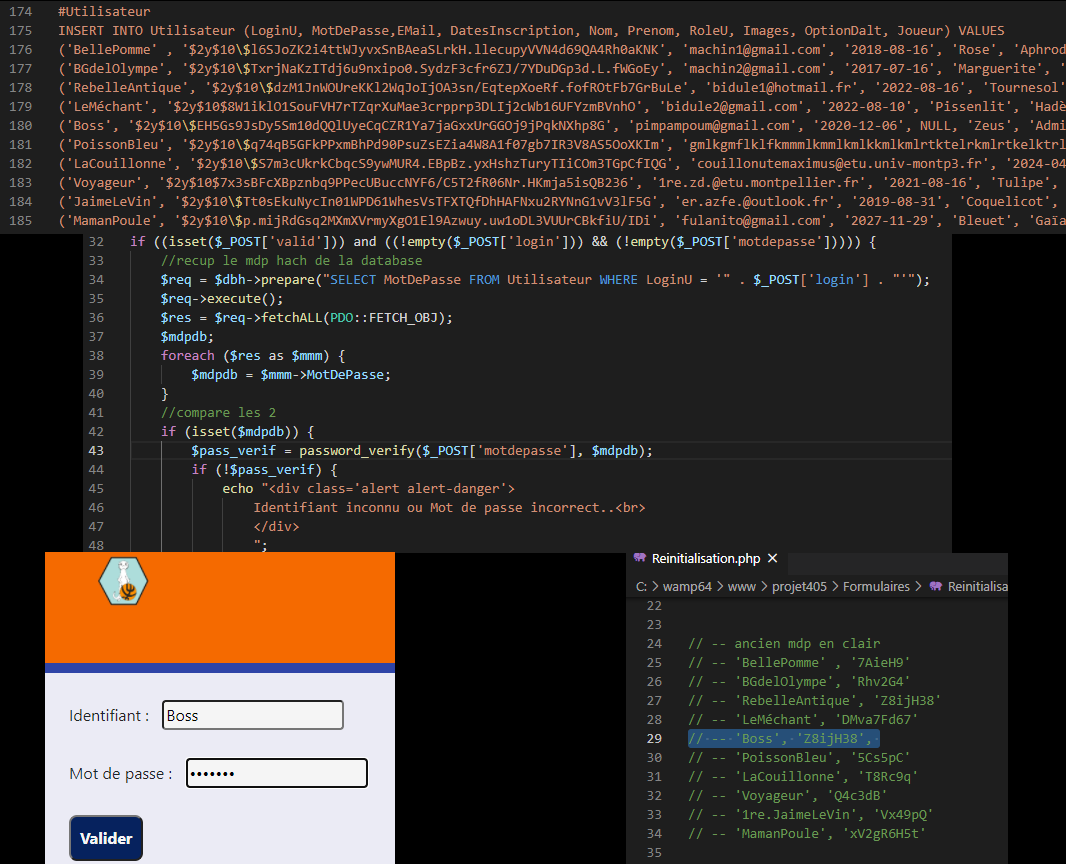
\includegraphics[height=12cm]{figures/pt-mdp.png}
			\caption{Hachage mot de passe}
\end{figure}
        \subsubsection{Démonstration}
\par                
La démonstration est en fait une réinitialisation de la BDD qui permet de détruire l’ensemble des tables, de les reconstruire et de réimplanter les exemples de bases nécessaires au développement des formulaires, puisque ces derniers les modifient. Le code comprend le SQL nécessaire ainsi qu’une redirection en JS, grâce à la fonction de stockage activée lors du clic sur le lien de la page Administrateur, aussi présente sur les liens de connexion. Si le développeur accède à ces pages par l’url sans clic préalable sur les liens activant les fonctions de stockage et que le stockage est de ce fait vide, une redirection vers l’accueil est prévue.
  
        \chapter{Conclusion}
        \par
        Dans ce rapport, nous avons expliqué comment nous avons géré notre travail d’équipe, construit notre base de données, mis en place l’architecture de notre site et ajouté des particularités techniques. Pour le conclure, il nous semble pertinent d’analyser et de comprendre ce qu’un tel projet nous a apporté en tant qu’élèves et futurs professionnels.\\Pour cela, nous allons aborder différents problèmes que nous avons pu rencontrer et la façon dont nous les avons traités et surmontés. Tout au long du projet, il a été important pour nous de ne pas voir ces épreuves, qu’elles soient techniques ou organisationnelles, comme des erreurs mais comme des tremplins de progression qui nous permettraient d’améliorer notre comportement en programmation à long terme. Cette perspective nous a permis de progresser et de ne pas rester bloqués face aux imprévus.
        \par
        Nous allons aborder ici trois situations épineuses auxquelles nous avons fait face : la découverte de l’inconnu, la difficulté de combiner cinq individualités et le défi de la normalisation. Ces trois sujets sur lesquels nous avons buté nous semblent intéressants, car ils regroupent à la fois des points relationnels et techniques et sont ceux qui nous ont le plus permis d’évoluer.
        
        \bigskip
        \par
        Premièrement, il a été assez difficile de se lancer dans un projet dans lequel tout ou presque semblait nouveau. À la première lecture, les consignes étaient assez longues et regorgeaient d’informations. Il nous paraissait précoce de mettre en place un calendrier de dates limites pour segmenter le travail puisqu’aucun de nous ne connaissait vraiment ce genre d’exercice. Il faillait trouver un moyen de s’y retrouver entre la nécessité de finir à temps et celle de fournir un travail complet.\\Au-delà de ces questionnements organisationnels, nous avons très vite compris que les cours portant sur le projet ne seraient pas suffisants pour tout coder. Ces cours étaient très récents et donc pas encore inscrits profondément dans nos mémoires. Après un an et demi d’informatique, nous savons qu’apprendre un langage ne se fait pas en regardant des gens programmer mais en programmant nous-mêmes. Face à la multiplicité de langages relativement nouveaux pour nous, nous avons donc rapidement su qu’il ne faudrait pas nous laisser déborder. En dehors des langages, le programme des cours qui devaient nous aider à structurer notre projet ne collait pas vraiment à notre calendrier.
        \par
        Nous sommes donc tous partis avec des a priori et des craintes qui auraient pu nous freiner si nous ne les avions pas mis en commun. Une des forces de notre équipe a été de beaucoup communiquer et de s’entraider à chaque étape complexe. Chacun s’est donc formé aux langages que nous devions utiliser, à travers les cours mais également grâce à des ressources trouvées en lignes, et a partagé ses connaissances afin de permettre à tous d’avancer. Nous avons aussi beaucoup utilisé nos outils de communication pour poser des questions auxquelles répondaient ceux qui le pouvaient. Enfin, les trois heures hebdomadaires de réunion ont parfois été utilisées pour permettre à chacun de “former” les autres.\\Cette façon de travailler nous a permis d’avancer efficacement, de prendre beaucoup d’initiatives et d’apprendre à travailler sans toujours suivre le chemin tracé d’un cours. Là où nous avions l’habitude d’avoir un cours magistral puis une séance de travaux dirigés associée, ce projet nous a permis d’apprendre à piocher dans les différentes banques de savoir à notre portée et de nous en servir pour avancer.
        \par
        Même si nous avons habilement réussi à dépasser nos incertitudes face à l’inconnu, notre tendance à prendre beaucoup d’initiatives a été source d’une nouvelle difficulté.
        
        \bigskip
        \par
        Deuxièmement, il a parfois été délicat de combiner les idées, les initiatives et les méthodes de travail de cinq personnes.
        \par
        Comme nous l’avons vu plus tôt, nous avons chacun appris du cours mais également de sources indépendantes. Ce système d’apprentissage et d’initiatives propre à chacun s’est révélé particulier à gérer. D’une part, générer son propre savoir et suivre ses propres idées empêche parfois d’être objectif et de différencier l’anecdotique du néccessaire, ce qui nous a poussés à nous acharner sur des détails techniques. D’autre part, s’est posé un problème organisationnel : être une équipe de cinq a autant d’avantages que d’inconvénients. En effet, plus le nombre de collaborateurs à un projet est grand, plus le nombre d’idées est important. Ainsi, une fois les premières étapes du projet passées, nous avions une liste d’idées supplémentaires débordante, et nous voulions tous voir nos propositions être exploitées. Nous avons donc dû faire des choix qui ne pourraient pas convenir à tout le monde puisque plus il y a d’opinions différentes, plus ces opinions peuvent être en opposition avec le choix de la majorité.
        \par
        La majorité est justement la méthode qui nous a permis de faire des choix équitables et communs. Nous nous sommes beaucoup servis de nos outils de communication pour que chacun puisse proposer un avis construit avant de voter et de choisir l’idée la plus fédératrice. Cette façon de faire a permis d’alléger les frustrations et de rester soudés jusqu’au bout sans que l’équipe ne se divise en plusieurs entités voulant emprunter des voies différentes. Nous avons également décidé de permettre à chacun de travailler sur les fonctionnalités supplémentaires qui l’intéressaient. Ainsi, nous avons tous pu suivre à la fois un chemin principal commun et passer plus de temps sur les notions qui nous intéressaient.
        \par
        En voyant les différents moments de désaccord et les solutions que nous avons mises en place, nous avons compris qu’il était particulièrement important pour une équipe de prendre des décisions fortes et d’y rester fidèle pour ne pas alimenter des débats déjà clos. C’est cette détermination qui nous a permis de ne pas nous attarder sur de nombreux points qui auraient pu nous retarder. Cependant, parmi ces points, il y a en a que nous avons abordés assez tard dans le projet : la normalisation des codes.
        
        \bigskip
        \par
        Troisièmement, normaliser les différents morceaux de codes pour les rendre lisibles par tous les membres et compatibles entre eux a été une étape complexe.
        \par
        Notre confrontation à la normalisation est la suite logique des deux difficultés précédentes. En effet, les initiatives nombreuses de chacun et le fait de manipuler des langages nouveaux pour nous nous ont freinés au moment de rendre les différents codes compatibles les uns avec les autres pour tous les relier. Puisque nous n’avions utilisé que très peu et très récemment les principaux langages du projet web, nous avons chacun développé nos propres habitudes et automatismes. Nous n’avions pas anticipé que ces automatismes propres à chacun pourraient être un obstacle à la réunification des codes, mais au moment d’assembler les codes et de regarder les productions des autres, nous nous sommes rendus compte du décalage.\\Hors de cet imprévu technique, normaliser nos approches organisationnelles et nos méthodes de travail été une grande partie du travail. Chacun des cinq membres a un parcours scolaire complètement différent et a donc engrangé des méthodes de travail différentes. De plus, un membre du groupe est en double licence, deux n’ont pas suivi une première année d’informatique, certains utilisent Windows et d’autres Linux, etc.
        \par
        Pour exploiter au mieux toutes ces différences, nous avons créé un cadre de travail commun permettant de conserver les particularités de chacun. Dans un contexte dans lequel nous ne nous sommes jamais rencontrés ou même vus, le concept de travail d’équipe semblait très abstrait. Nous avons donc beaucoup exploité les temps de réunion pour nous mettre d’accord sur les normes que nous appliquerions pour construire la structure du site, nous avons également appris à travailler en nous adaptant les uns aux autres.\\Ces étapes primordiales, bien que tardivement réalisées, nous ont permis de faciliter la mise en commun et le débogage puisque chacun connaissait et comprenait le travail des autres. Par-dessus tout, ce qui aurait pu sembler être une erreur rédhibitoire pour la suite du projet nous a permis d’apprendre à mieux prévoir et anticiper les potentiels décalages afin de ne plus en subir les conséquences.
        \bigskip
        \par
        Les nombreuses semaines pendant lesquelles nous avons travaillé sur ce projet nous ont permis d’apprendre la gestion du temps et la pression, le travail de groupe dans un environnement et un contexte quasiment inconnu, et par-dessus tout la prise d’initiatives et de décisions à plusieurs. Au-delà des langages que nous avons appris à connaître plus en profondeur, nous avons surtout su retenir de ce projet qu’au sein d’une équipe, la collaboration est la clé de la réussite.

		\chapter{Annexe}

	    %annexe intro
	    
	    %annexe gestion de groupe
	    \section {Gestion de groupe}
	     \begin{figure}[!h]
			\centering
				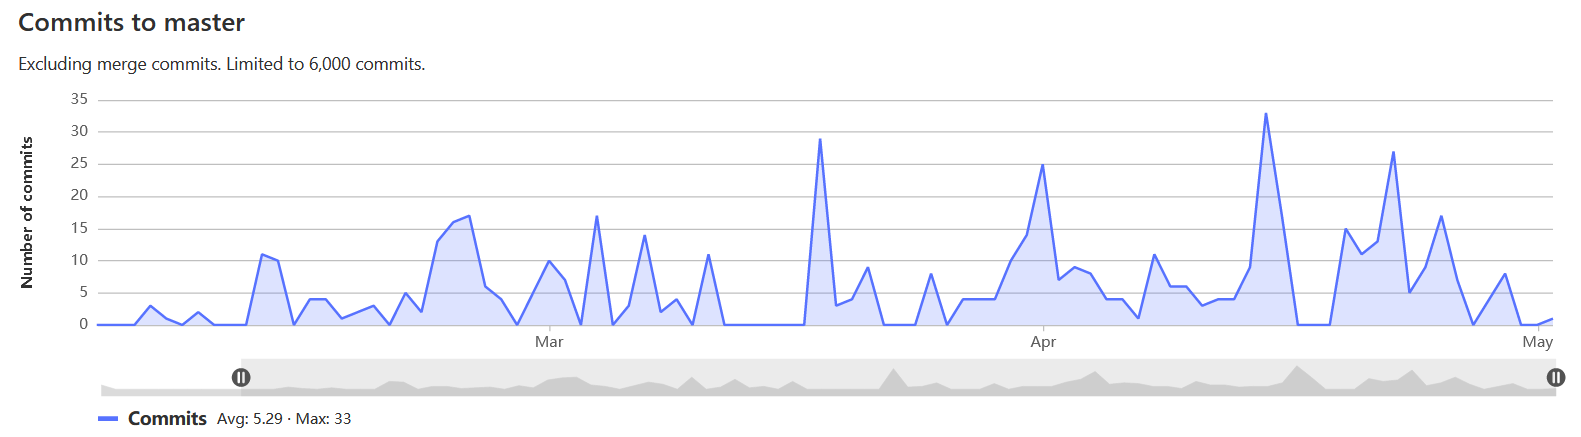
\includegraphics[height=5cm]{figures/bdd-rapport-5.PNG}
			\caption{Graphique de la quantité de "commits" sur le projet}
		\end{figure}
	    \hypertarget{annexe-gestion}{}

	    \begin{figure}[!h]
			\centering
				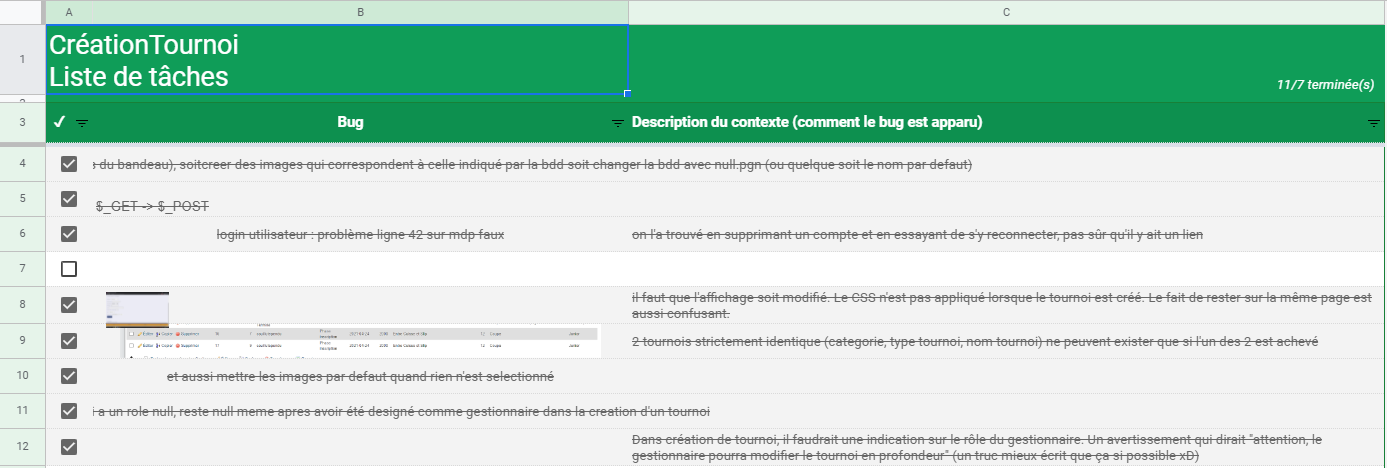
\includegraphics[height=6cm]{figures/bdd-rapport-4.PNG}
			\caption{Tableur de bugs sur le formulaire de création de tournoi manuelle}
		\end{figure}
	    \begin{figure}[!h]
			\centering
				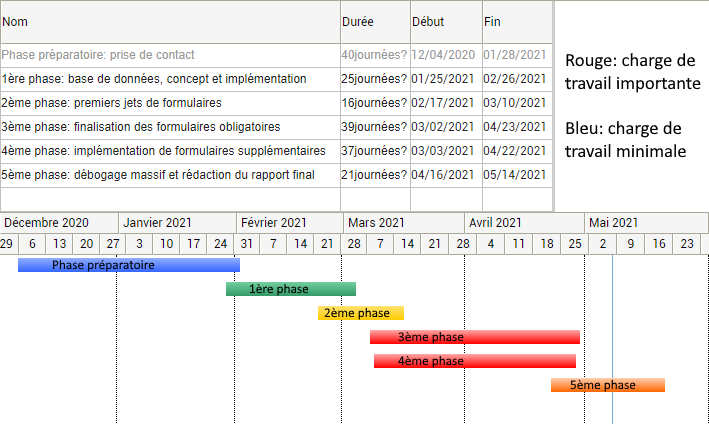
\includegraphics[height=10cm]{figures/bdd-rapport-gantt.png}
			\caption{Diagramme de Gantt du déroulement des phases du projet}
		\end{figure}
		\newpage
		\hyperlink{bdd-retour-gestion}{Revenir à la gestion de groupe}
		
	    %annexe base de données
	    \newpage
        \section {Base de données}
 
	    \hypertarget{annexe-bdd-tableref}{}
	    
	    \begin{figure}[!h]
			\centering
				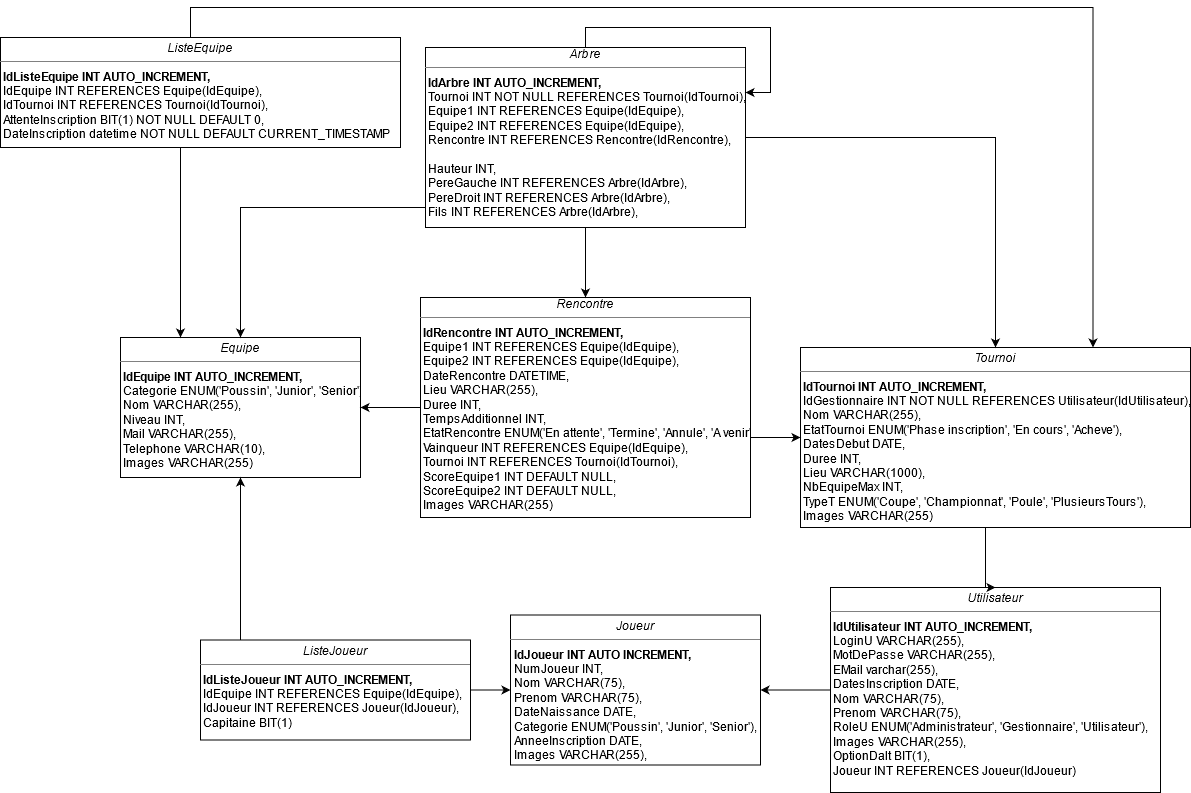
\includegraphics[height=12cm]{figures/bdd-rapport-3-meerkat.png}
			\caption{Table de référence pour la base de donnée}
		\end{figure}
		\hyperlink{bdd-retour-annexe}{Revenir à la mise en place de la base de données}
		\bigskip
		
	     %annexe architecture
	    
	    %annexe particularités techniques
	    \newpage
        
	    \section {Accessibilité et autorisations}
	    \hypertarget{annexe-access-et-auto}{}
\par
L’utilisation de PDO permet l’appel dans le bandeau et dans les formulaires de la même BDD, simultanément et sans compromettre son intégrité, ce que ne permet pas mysqli, et qui nous aurait obligés à être encore plus normatifs quant au nommage de la connexion vers la BDD, pour permettre de gérer au mieux les exceptions. En effet, a été mise en place une connexion commune pour les administrateurs (\hyperlink{fig-connexion}{Connexion BDD}), où seul le nom de la variable qui stocke la connexion est autorisé à changer ; les autres variables internes sont fournies par l’inclusion du fichier connexion.php où chaque administrateur aura renseigné ses identifiants et mot de passe utilisées pour se connecter à phpmyadmin.
 \begin{figure}[h]
 				\hypertarget{fig-connexion}{}
			\centering
				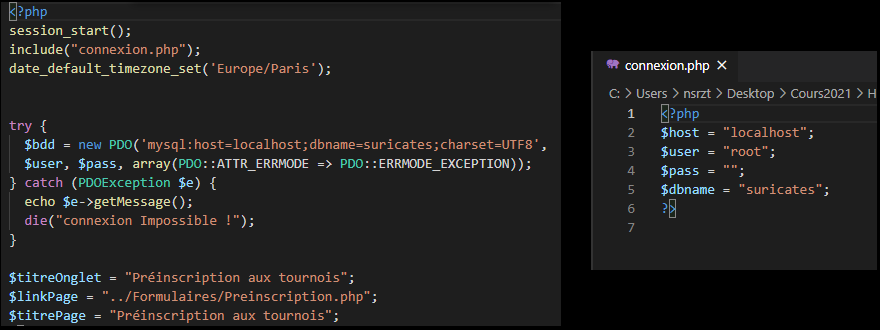
\includegraphics[height=5cm]{figures/pt-connexionbdd.png}
			\caption{Connexion BDD}
\end{figure}
\par
Les fonctions isset et empty ont été particulièrement utiles (\hyperlink{fig-issetempty}{Isset, empty}), du fait de la redirection sur l’url courante de bon nombre de formulaires. Il fallait prévoir les affichages différents selon la présence de certaines variables, en plus de gérer les autorisations d’accès, en fonction des rôles, qui ont été introduites avant la création de l’espace membre et de la facilitation qu’offre le stockage des ID et rôles dans la super globale SESSION. Il en découle des requêtes et des vérifications qui ne sont plus optimales mais qui sont intimement liées les unes les autres, du fait d’une conception précoce des formulaires. L’utilisation en matrice de plusieurs dimensions de la super globable SESSION permet de réduire les probabilités au sein d’un groupe de développeurs d’utiliser un même nom et d’écraser par inadvertance ou par effet de bord le contenu.
 \begin{figure}[h]
 \hypertarget{fig-issetempty}{}
			\centering
				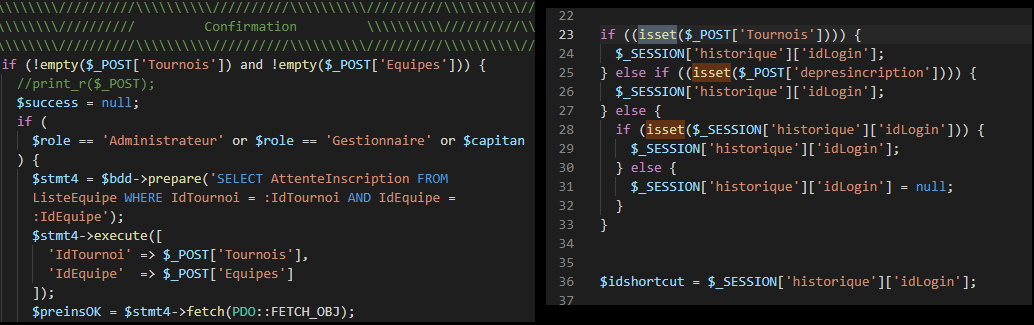
\includegraphics[height=5cm]{figures/pt-issetempty.png}
			\caption{Isset, empty}
\end{figure}
\bigskip
\par
\hyperlink{retour-access-auto}{Revenir aux particularités techniques}
 \section {Unifier l’application Web}
 \hypertarget{annexe-unifier-web}{}
\par
Dans le répertoire CadreStatique, les fichiers skel1.php et skel2.php sont la condensation de dizaines d’autres fichiers originellement introduits par la fonctionnalité include de php et qui nous ont amenés à revoir la conception html du header (l’imbrication des div…), de la navigation et du bandeau latéral. Bien plus complexe de base, il était urgent de factoriser et simplifier le code pour que chacun puisse participer à l’unification des différents formulaires en une unique application web. Dorénavant, chaque nouvelle page est créée sur le modèle du squelette.php (\hyperlink{fig-squelette}{Squelette.php}),
fichier modèle dans lequel le contenu est introduit entre les éléments essentiels et/ou factorisés
comme le header, etc.
 \begin{figure}[h]
 				\hypertarget{fig-squelette}{}
			\centering
				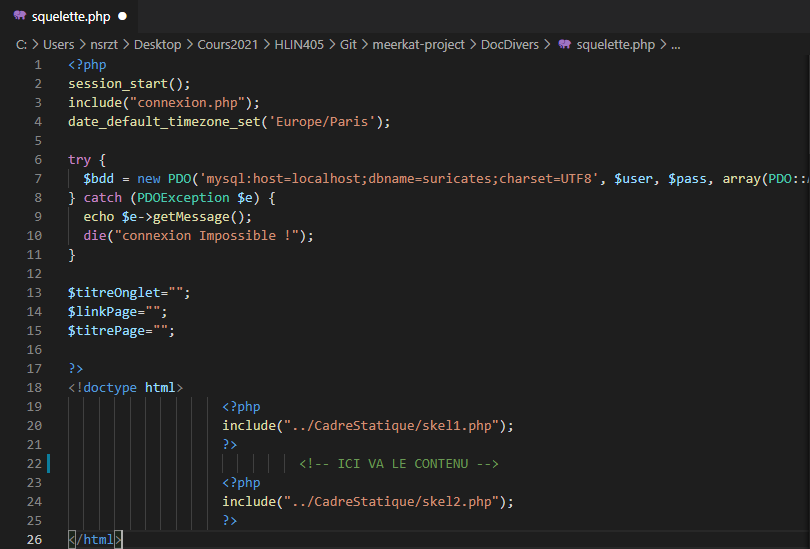
\includegraphics[height=9cm]{figures/pt-squelette.png}
			\caption{Squelette.php}
\end{figure}
\bigskip
\par
\hyperlink{retour-unifier}{Revenir aux particularités techniques}
\newpage
	    \section {Rendu visuel (+ responsive)}
	    \hypertarget{annexe-rendu-visuel}{}
\par
Le framework Bootstrap a été introduit, tout comme d’autres éléments externes tels que les librairies JS, le plus souvent pour une fonctionnalité particulière et le responsive des classes colonnes. Son utilisation a été dans l’ensemble un frein à la conception graphique du fait de la non maîtrise de base des langages HTML et CSS. En effet, des propriétés de bases propres aux marges, aux blocs ont rendu difficile l’alignement des éléments, couplées à l’imbrication des éléments et des propriétés d’héritages en cascade. Avec la factorisation du code, ce sont les principales raisons qui nous ont amenés à diverger du mockup (\hyperlink{fig-mockup}{Mockup}).
\begin{figure}[h]
\hypertarget{fig-mockup}{}
			\centering
				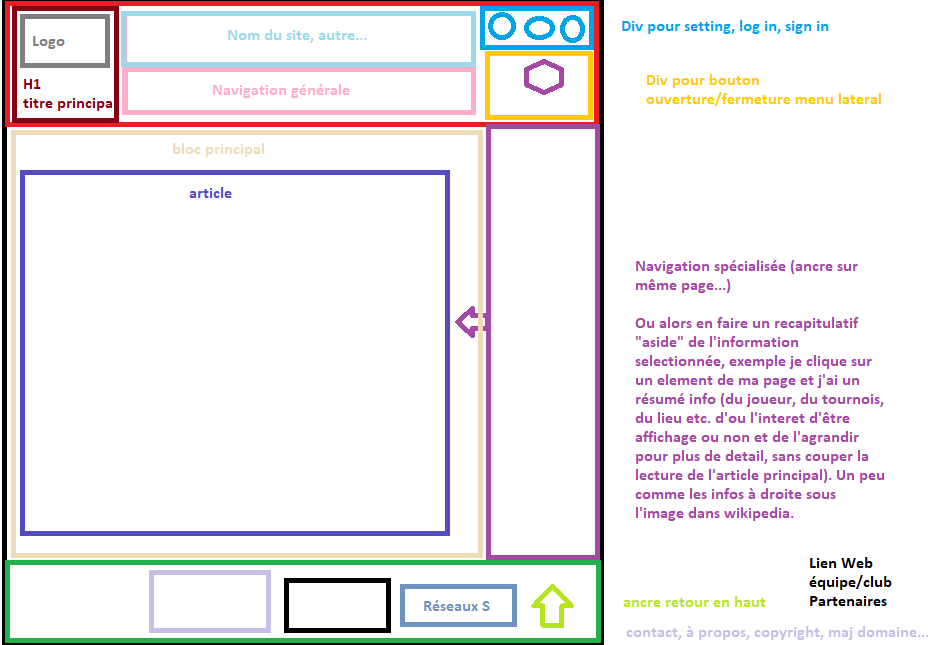
\includegraphics[width=17cm]{figures/pt-mockup.png}
			\caption{Mockup}
\end{figure}
\bigskip
\par
Seul le strict minimum au niveau librairie a été conservé, et ce sont relativement les plus volumineux de nos fichiers ; de plus il s’agit de la version 5 de Bootstrap, une version beta. De ce fait, nous avons rencontré des difficultés à mettre en place toutes les fonctionnalités des carrousels, il fallait en fait reprendre des librairies de la version antérieure pour que les flèches latérales (les contrôleurs) ou même que les indications caudales de positionnement apparaissent. Un deuxième type de carrousel a ensuite été introduit, celui à 5 images visibles, plus esthétique mais presque entièrement fourni par une librairie, contrairement au premier, qui lui est codé entièrement par nos soins. Le premier carrousel (à une seule image) s’est donc vu relayé à l’affichage responsive des petits écrans (remplace celui à 5 images) ainsi que pour le contenu du bandeau latéral où les multiples carrousels ont en plus été épurés des contrôleurs/indicateurs.
\bigskip
\par
\begin{wrapfigure}{l}{0.6\textwidth}
\hypertarget{fig-media}{}
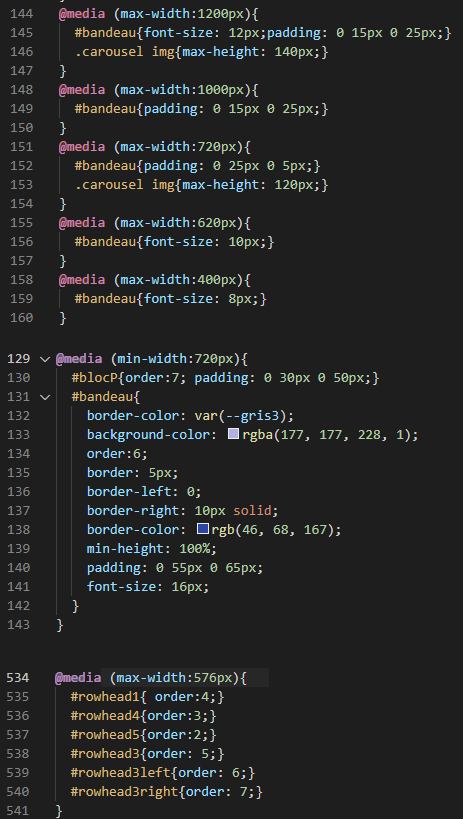
\includegraphics[width=0.9\linewidth]{figures/pt-media.png}
\caption{Media}
\end{wrapfigure}
Il a fallu rendre par la suite tout le site responsive, et en particulier les éléments factorisés. Les classes img-fluid ont été particulièrement utiles pour les images des carrousels, chapotées par des propriétés de position, de max height, de width auto, etc. L’atout particulier de notre code CSS en matière de responsive est l’utilisation de @media (\hyperlink{fig-media}{Media}) qui complète le maillage (grid) de bootstrap (col-sm-12…). Différentes tailles d’écran ont été étudiées et l’ordre des éléments html s’est vu modifié grâce au CSS (propriété order). La taille des images, des polices sont ajustées à chaque définition ainsi que le positionnement du bandeau latéral à gauche pour les ordinateurs/tablettes et à droite de l’article principal pour les plus petits écrans (en raison de la prévalence de droitiers dans la population et de l’utilisation du pouce sur les téléphones).
\bigskip
\par
Enfin, a été mise en place une version dite « daltonienne » du CSS, qui consiste à griser de façon réfléchie les couleurs pour obtenir des nuances de gris contrôlées et empêcher qu’un effet/élément disparaisse du spectre de vision des personnes atteintes de dyschromatopsie (voir Charte Graphique). Cet effet est disponible dès l’inscription, modifiable en option de compte, et repose sur le principe que la dernière inclusion CSS prime, donc son inclusion est faite postérieurement au style.css principal en fonction d’une condition issue d’une requête PHP.
\bigskip
\par
\hyperlink{retour-rendu-visuel}{Revenir aux particularités techniques}
\newpage
	    \section {Formulaires}
	    \hypertarget{annexe-formulaires}{}
\begin{wrapfigure}{h}{0.6\textwidth}
\hypertarget{fig-requete}{}
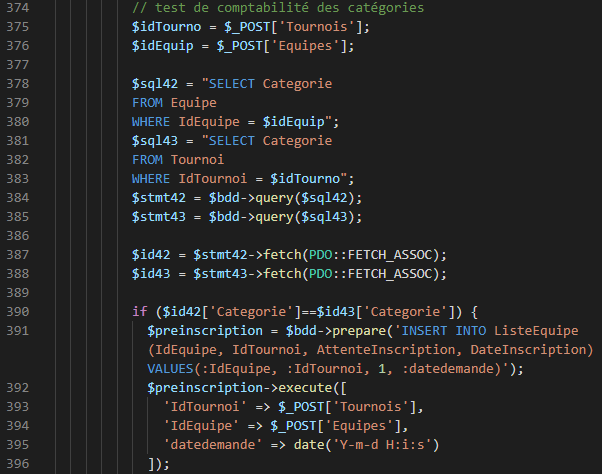
\includegraphics[width=0.9\linewidth]{figures/pt-requete.png}
\caption{Requête}
\end{wrapfigure}
\par
Les différentes requêtes sont effectuées en passant par PDO, au moyen de query, exec, prepare suivi de execute puis l’extraction est faite en utilisant fetch/fetchall et FETCH\_ASSOC ou OBJ puis while ou foreach. Il a été très utile de passer les requêtes dans des variables avant leur exécution, le tout entre simples quotes ‘ et non pas entre doubles quotes, pour permettre l’interprétation d’autres variables, avec comme inconvénient que les variables comportant des quotes comme peuvent l’être les \$\_POST[‘var’] ne sont pas déspécialisables, il faut donc les affecter dans des variables aux noms plus standards (\hyperlink{fig-requete}{Requête}).
\bigskip
\par
Les formulaires utilisent les fonctionnalités basiques select avec des boucles affichant les données préalablement extraites depuis la BDD (Fig X : Select); mais aussi des input de type text avec des sécurités sur les regex, du traitement de symboles, des options required, placeholder ou disabled, la sauvegarde des entrées en cas d’erreur pour ne pas avoir à tout réécrire ou rappeler les précédents choix (\hyperlink{fig-select}{Select - Ligne 195}), des roulettes pour les numéros, du formatage de date avec date actuelle de base, date minimale en cas d’absence etc (\hyperlink{fig-input}{Input}).
\begin{figure}[h]
\hypertarget{fig-select}{}
			\centering
				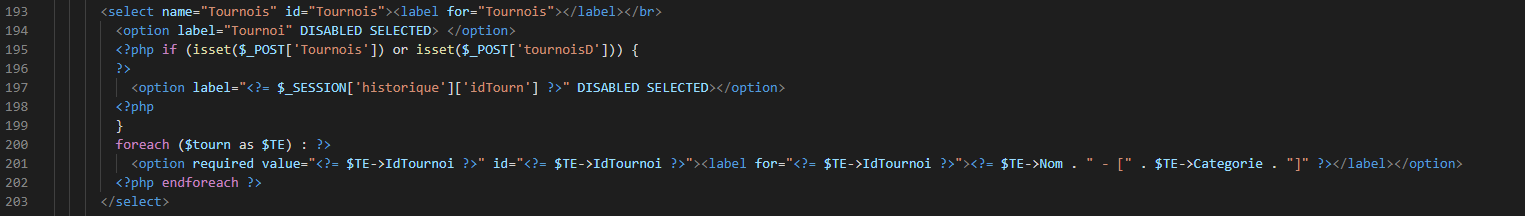
\includegraphics[width= 17cm]{figures/pt-select.png}
			\caption{Select}
\end{figure}

\begin{figure}[h]
\hypertarget{fig-input}{}
			\centering
				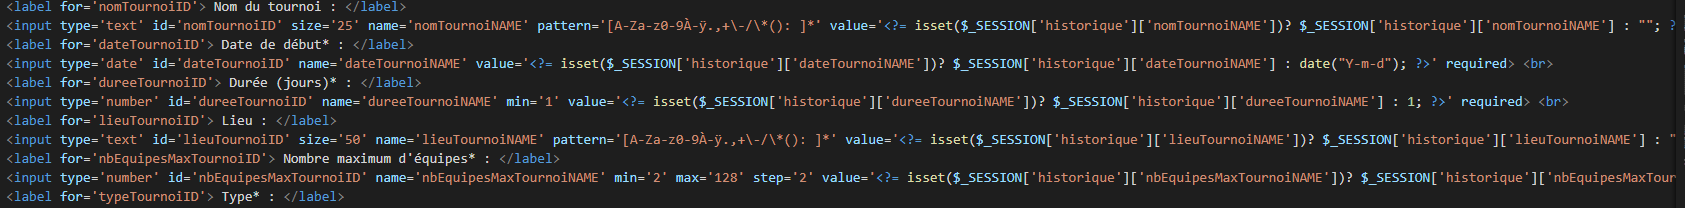
\includegraphics[width= 17cm]{figures/pt-input.png}
			\caption{Input}
\end{figure}
\bigskip
\par
Pour faire un select à n valeurs venant d’un array/objet servant à stocker les données de la requêtes SQL précédente, il faut en principe écrire en pseudo code : value = « \$nième valeur ». Or, le form est en html, et pour passer une telle variable il fallait repasser (switcher) en PHP et empêcher la déspécialisation du \$, des balises et du ?. Cependant, il est impossible de passer < ?php après de simples/doubles quotes du HTML. Il fallait donc contourner le problème en utilisant une balise ouvrante raccourcie < ?= qui elle n’est pas refusée et permet de switcher PHP/HTML à l’intérieur des doubles quotes du value. La balise fermante ?> étant la même dans les deux cas. (\hyperlink{fig-select}{Select - Ligne 201}). Quand bien même cette astuce marche in vitro sur WAMP, mais ces balises appartiennent à d’autres langages tels que XML, et les serveurs disposent de protections contre les injections et pour se prémunir, retirent les options de balises raccourcies que nous propose la config local de PHP. En conséquence, il est probable que certains serveurs ne reconnaissent plus notre code, l’interprétant dans le mauvais langage. Séparer tous les codes HTML du PHP, comme le proposent les architectures MVC pourrait être une solution mais la configuration actuelle est limitante : il est difficile d’adopter cela en groupe, après plusieurs semaines de travail, et jusqu’alors non étudiée.
\bigskip
\par
\hyperlink{retour-formulaires}{Revenir aux particularités techniques}
\newpage
	    \section {Bandeau}
	    \hypertarget{annexe-bandeau}{}
\par
Le bouton bandeau est déplaçable n’importe où sur la page, en dehors même de sa div, à la façon d’un drag and drop. Il possède aussi la fonctionnalité de faire disparaitre le bandeau latéral comme son nom le suggère, tout en conservant ce choix d’une page à l’autre. Le contenu du bandeau est celui des prochains évènements (rencontres sportives), le bouton principal (évènements) déplie les autres pour tout afficher en un instant, de plus chacune des sous-parties possède son propre bouton de déploiement.
\bigskip

\begin{wrapfigure}{l}{0.5\textwidth}
\hypertarget{fig-balise-body}{}
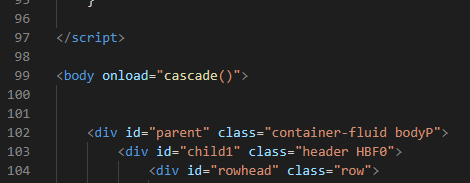
\includegraphics[width=0.95\linewidth]{figures/pt-balisebody.png}
\caption{Balise body}
\hypertarget{fig-js}{}
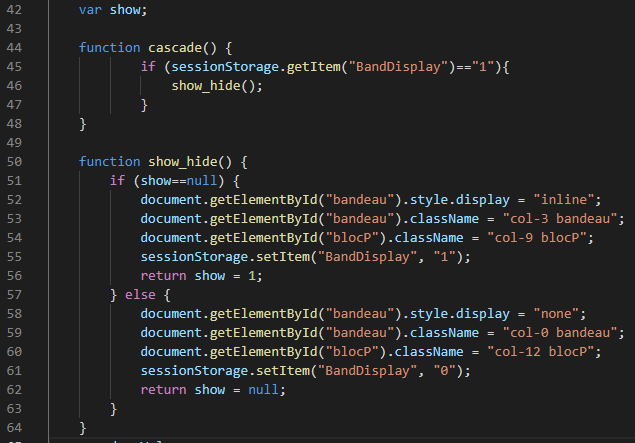
\includegraphics[width=0.95\linewidth]{figures/pt-js.png}
\caption{Javascript}
\hypertarget{fig-bouton-bandeau}{}
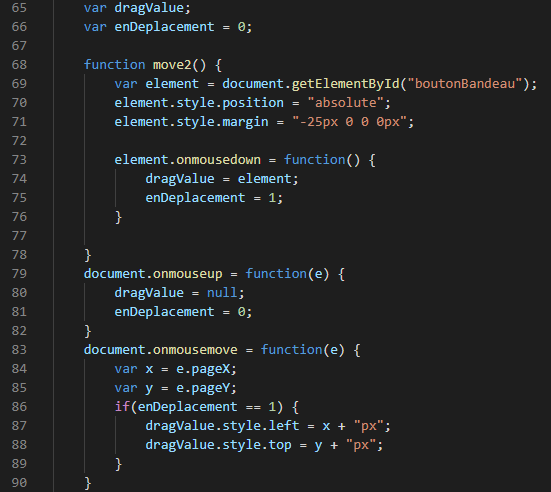
\includegraphics[width=0.95\linewidth]{figures/pt-btnbandeau.png}
\caption{Bouton bandeau}
\end{wrapfigure}
\par
La fonction cascade (skel1.php) (\hyperlink{fig-balise-body}{Balisebody}) est un reliquat des précédentes implémentations, comme il n’est pas possible de placer plus d’une seule fonction au lancement d’une page avec onload dans la balise body. Cette fonction appelle toutes les fonctions, elle a été conservée par la suite, dans l’éventualité d’autres ajouts, bien que ne comportant qu’une seule fonction de démarrage au chargement, actuellement.
\newline
\bigskip
\par
Via JS, le CSS est modifié, en particulier le style display qui alterne entre none et inline/block pour l’affichage, de même que la classe peut être éditée comme c’est le cas des fonctions qui affectent le bandeau et l’article principal pour rééquilibrer l’affichage en col-3 et col-9 ou col-12 \hyperlink{fig-js}{Javascript} ou même les onglets, ce qui est l’équivalent de la fonction toggle.
\bigskip
\newline
\bigskip
\par
La fonctionnalité de drag du bouton bandeau, à travers toute la page, (\hyperlink{fig-bouton-bandeau}{bouton bandeau}) est permise par 3 fonctions et 2 variables locales, dragValue sert à agir sur la position (pageX/Y, style.left/top) tandis que enDeplacement sert à contrôler les appels aux fonctions, le tout couplé aux fonctions JS qui interagissent avec la souris (onmouseup/down).
\bigskip
\par
\hyperlink{retour-bandeau}{Revenir aux particularités techniques}


\end{document}